\chapter{Particle-Based Simulations}
\label{chapter particle}



Besides the grid-based fluid simulations algorithms, this project also studied and implemented a fundamentally different algorithm, known as \textbf{PBF} (Position-Based Fluids), which only uses particles to represent the fluid and its relevant scalar and vector fields. The principles of this algorithm is given in this chapter.


\section{Smoothed Particle Hydrodynamics}
PBF belongs to a family of algorithms called SPH(Smoothed Particle Hydrodynamics). SPH does not utilize a grid to discretize scalar and vector fields, and instead only uses a large cloud of particles to represent to the fluid. All quantities that are involved in the simulation are carried by these particles. For some quantity $Q$, either scalar or vector, and some location $\textbf{x}$, SPH approximates $Q$ at $Q(\textbf{x})$ as a weighted average of $Q$ carried by the nearby particles.
\begin{equation}
    \label{eqn SPH basic}
    \begin{aligned}
        Q(\textbf{x}) = \sum_{j=1}^N m_j \frac{Q_j}{\rho_j} W(\textbf{x}-\textbf{x}_j,h)
    \end{aligned}
\end{equation}
where $N$ is the total amount of particles, $m_j$ is the mass of the $j$th particle, $\textbf{x}_j$ its position, $\rho_j$ its density, and $Q_j$ the value of $Q$ it carries. Most importantly, $W$ is a \textit{smoothing kernel function}, and $h$ its \textit{smoothing radius}, which satisfies the properties:
\begin{equation}
    \begin{aligned}
        \forall\textbf{r}~~s.t~~||\textbf{r}||>h, W(\textbf{r},h) &= 0\\
        \int W(\textbf{r},h) d\textbf{r} &= 1
    \end{aligned}
\end{equation}
$W$ is used to decide the contribution weight of each particle, which is greater if $\textbf{x}_j$ is closer to $\textbf{x}$. Thus, normally the value of $W(\textbf{r},h)$ only depends on $||r||$, and is $0$ if $||r||>h$.


A convenient and important property of the SPH framework is that, computing the gradient/Laplacian of a quantity can be done by only applying the gradient/Laplacian operator on the smoothing kernel:
\begin{equation}
    \label{eqn SPH derivative}
    \begin{aligned}
        \nabla Q(\textbf{x}) &= \sum_{j} m_j \frac{Q_j}{\rho_j} \nabla W(\textbf{x}-\textbf{x}_j,h) \\
        \nabla \cdot \nabla Q(\textbf{x}) &= \sum_{j} m_j \frac{Q_j}{\rho_j} \nabla \cdot \nabla W(\textbf{x}-\textbf{x}_j,h)
    \end{aligned}
\end{equation}
A common choice of $W$ is the ``poly6" function:
$$
    W_{poly6}(\textbf{r},h)=
        \begin{cases}
            \frac{315}{64\pi h^9}(h^2-||\textbf{r}||^2)^3 &\mbox{ if } 0\leq||\textbf{r}||\leq h\\
            0 &\mbox{otherwise} 
        \end{cases}
$$
However, this function has the problem that, its gradient vanishes as $\textbf{r}$ approaches $\textbf{0}$. Thus, when computing $\nabla W$, a alternative kernel called the ``spiky" kernel is used:
$$
    \nabla W_{spiky}(\textbf{r},h)=
        \begin{cases}
            \frac{-45}{\pi h^6||\textbf{r}||}(h-||\textbf{r}||)^2\textbf{r} &\mbox{ if } 0\leq||\textbf{r}||\leq h\\
            \textbf{0} &\mbox{otherwise} 
        \end{cases}
$$
The following figure illustrates the difference between the two kernels:

\begin{figure}[H]
    \label{figure kernels}
    \begin{tikzpicture}
        \draw[->] (-3,0) -- (4.2,0) node[right] {$x$};
        \draw[->] (0,-3) -- (0,4.2) node[above] {$y$};
        \draw[scale=1.0,domain=-1:1,smooth,variable=\x,blue,line width=0.25mm] plot ({\x},
           {(1-\x*\x)*(1-\x*\x)*(1-\x*\x)}
        );
        \draw[scale=1.0,domain=-1:1,smooth,variable=\x,red,dashed,line width=0.25mm] plot ({\x},
           {-6*(1-\x*\x)*(1-\x*\x)*\x}
        );
        \draw[blue,line width=0.25mm] (1.5,2.5) -- (2,2.5) node[right] {$W_{poly6}$};
        \draw[red,dashed,line width=0.25mm] (1.5,2) -- (2,2) node[right] {$\nabla W_{poly6}$};
      \end{tikzpicture}
      \begin{tikzpicture}
        \draw[->] (-3,0) -- (4.2,0) node[right] {$x$};
        \draw[->] (0,-3) -- (0,4.2) node[above] {$y$};
        \draw[scale=1.0,domain=-1:1,smooth,variable=\x,blue,line width=0.25mm] plot ({\x},
           {(1-abs(\x))*(1-abs(\x))*(1-abs(\x))}
        );
        \draw[scale=1.0,domain=0:1,smooth,variable=\x,red,dashed,line width=0.25mm] plot ({\x},
           {-3*(1-\x)*(1-\x)}
        );
        \draw[scale=1.0,domain=-1:0,smooth,variable=\x,red,dashed,line width=0.25mm] plot ({\x},
           {3*(1+\x)*(1+\x)}
        );
        \draw[blue,line width=0.25mm] (1.5,2.5) -- (2,2.5) node[right] {$W_{spiky}$};
        \draw[red,dashed,line width=0.25mm] (1.5,2) -- (2,2) node[right] {$\nabla W_{spiky}$};
      \end{tikzpicture}

      \caption{Scalar versions of $W_{poly6}$ and $W_{spiky}$}
      
\end{figure}

In the first paper where SPH is used for computer graphics, written by Matthias Müller\cite{muller2003particle} in 2003, each quantity involved in the Navier-Stokes momentum equation is explicitly written in the forms of formula \ref{eqn SPH basic} or \ref{eqn SPH derivative}. An explicit time stepping integration is then used to update the velocity field and particle positions. However, the incompressibility condition was ignored in that paper. Since then, many extensions and modifications to the original SPH scheme was proposed, which enforces incompressibility. The newest and currently most popular one of these extensions is proposed in 2013, again developed by Müller and his colleague Macklin in NVIDIA\cite{macklin2013position}. This extension is the Position Based Fluids algorithm.


\section{Position Based Fluids}
In Position Based Fluids, or PBF, the incompressibility condition is enforced by putting an explicit constraint on the density of the fluid. To begin with, for each particle $i$ at position $\textbf{x}_i$ the density at each particle can be derived using formula \ref{eqn SPH basic}:
\begin{equation*}
    \begin{aligned}
        \rho_i &= \sum_{j} m_j \frac{\rho_j}{\rho_j} W(\textbf{x}_i-\textbf{x}_j,h)\\
        &= \sum_{j} m_j W(\textbf{x}_i-\textbf{x}_j,h)
    \end{aligned}
\end{equation*}
PBF treats all particles as having equal mass. This mass can be chosen to be $1$, which simplifies the formula:
\begin{equation}
    \label{eqn PBF rho}
    \begin{aligned}
        \rho_i 
        &= \sum_{j} W(\textbf{x}_i-\textbf{x}_j,h)
    \end{aligned}
\end{equation}
Note that $\rho_i$ is in fact a function of the positions of all the particles in the simulation: $\rho_i = \rho_i(\textbf{x}_0,\textbf{x}_1,\dots,\textbf{x}_N)$ where $N$ is the total amount of particles. Using the density of each particle, PBF defines a constraint quantity $C_i$ for each particle $i$:
$$
C_i(\textbf{x}_0,\textbf{x}_1,\dots,\textbf{x}_N) = \frac{\rho_i}{\rho_{rest}} - 1
$$
where $\rho_{rest}$ is the rest density of the fluid. The incompressibility constraint can then be explicitly written as:
$$
C_i(\textbf{x}_0,\textbf{x}_1,\dots,\textbf{x}_N) = 0
$$
Collectively, using the concatenated vector $\textbf{X} = [\textbf{x}_1^T,\textbf{x}_2^T,\dots,\textbf{x}^T]^T$ to denote the positions of all particles, the constraint of the $i$th particle can be written as:
\begin{equation}
    C_i(\textbf{X}) = 0
\end{equation}

In each time step of the PBF simulation, the algorithm begins by predicting a new position $\textbf{x}_i^*$ for each particle $i$ using its velocity $\u_i$:
$$
\textbf{x}_i^* = \textbf{x}_i + \triangle t \u_i
$$
If the particle happens to travel into a solid region, some basic collision handling should also be applied (e.g clamping $\textbf{x}_i^*$ outside the solid).

Let $\textbf{X}^*=[\textbf{x}_1^{*T},\textbf{x}_2^{*T},\dots,\textbf{x}_N^{*T}]^T$ be the collective predicted position, then, in all likelihood, $\textbf{X}^*$ will not satisfy the density constraints. Thus, PBF aims to find a set of corrections for the particles' positions, $\triangle\textbf{X}=[\triangle\textbf{x}_1^T,\triangle\textbf{x}_2^T,\dots,\triangle\textbf{x}_N^T]^T$, which restores the density constraints:
\begin{equation}
    \label{eqn density constrain C(x+dx)=0}
    C_i(\textbf{X}^* + \triangle\textbf{X}) = 0~~\forall i \in [0\dots N]
\end{equation}
PBF approximates $\triangle\textbf{X}$ by restricting it in the direction of $\nabla C_i(\textbf{X}^*)$:
\begin{equation}
    \begin{aligned}
        \triangle\textbf{X} \approx  \lambda_i \nabla C_i(\textbf{X}^*)
    \end{aligned}
\end{equation}
where $\lambda_i$ is a scalar coefficient. To find a suitable $\lambda_i$, PBF considers the 1st order Taylor series of $C_i(\textbf{X}^* + \triangle\textbf{X})$:
\begin{equation}
    \begin{aligned}
        C_i(\textbf{X}^* + \triangle\textbf{X}) 
        &\approx  C_i(\textbf{X}^*) + (\nabla C_i(\textbf{X}^*))^T \triangle\textbf{X} \\
        &\approx  C_i(\textbf{X}^*) + (\nabla C_i(\textbf{X}^*))^T  \nabla C_i(\textbf{X}^*) \lambda_i \\
        &=  C_i(\textbf{X}^*) + ||\nabla C_i(\textbf{X}^*)||^2  \lambda_i
    \end{aligned}
\end{equation}
Combining this with formula \ref{eqn density constrain C(x+dx)=0}, it can be derived that
\begin{equation}
    \label{eqn lambda i basic}
    \begin{aligned}
        \lambda_i &\approx \frac{-C_i(\textbf{X}^*)}{||\nabla C_i(\textbf{X}^*)||^2}\\
        &= \frac{-C_i(\textbf{X}^*)}{ \sum_{j} ||\nabla_{\textbf{x}^*_j} C_i(\textbf{X}^*)||^2}
    \end{aligned}
\end{equation}
The summation in the denominator can be separated into two cases: when $j=i$ and $j\neq i$
\begin{equation}
    \label{eqn lambda i expanded}
    \begin{aligned}
        \lambda_i  \approx\frac{-C_i(\textbf{X}^*)}{ ||\nabla_{\textbf{x}^*_i} C_i(\textbf{X}^*)||^2 + \sum_{j\neq i} ||\nabla_{\textbf{x}^*_j} C_i(\textbf{X}^*)||^2}\\
    \end{aligned}
\end{equation}
And then the SPH formula for gradients \ref{eqn SPH derivative} can be used to explicit compute each term:
\begin{equation*}
    \begin{aligned}
        \nabla_{\textbf{x}^*_i} C_i(\textbf{X}^*) 
        &= \frac{1}{\rho_{rest}}\sum_j \nabla_{\textbf{x}^*_i} W (\textbf{x}^*_i - \textbf{x}^*_j,h)\\
        &= \frac{1}{\rho_{rest}}\sum_j \nabla W (\textbf{x}^*_i - \textbf{x}^*_j,h)
        \\
        \nabla_{\textbf{x}^*_j} C_i(\textbf{X}^*) 
        &= \frac{1}{\rho_{rest}}\nabla_{\textbf{x}^*_j} W (\textbf{x}^*_i - \textbf{x}^*_j,h)\\
        &= \frac{-1}{\rho_{rest}}\nabla W (\textbf{x}^*_i - \textbf{x}^*_j,h)
    \end{aligned}
\end{equation*}
Substituting these back into formula \ref{eqn lambda i expanded} gives
\begin{equation}
    \label{eqn lambda i final}
    \begin{aligned}
        \lambda_i  &\approx\frac{-C_i(\textbf{X}^*)}{ 
            \frac{1}{\rho_{rest}^2} (||\sum_j \nabla W (\textbf{x}^*_i - \textbf{x}^*_j,h)||^2 + \sum_j ||\nabla W (\textbf{x}^*_i - \textbf{x}^*_j,h)||^2)
        }\\
        &=\frac{-(\frac{\rho_i}{\rho_{rest}}-1)}{ 
            \frac{1}{\rho_{rest}^2} (||\sum_j \nabla W (\textbf{x}^*_i - \textbf{x}^*_j,h)||^2 + \sum_j ||\nabla W (\textbf{x}^*_i - \textbf{x}^*_j,h)||^2)
        }
    \end{aligned}
\end{equation}
which is now in a form ready to be translated into CUDA code.

Having obtained $\lambda_i$ for each particle constraint $C_i$, the corrections to particle locations can be computed as a sum of the corrections from all constraints:
\begin{equation}
    \label{eqn PBF delta x}
    \begin{aligned}
        \triangle \textbf{x}_i 
        &= \sum_{j} \lambda_j \nabla_{\textbf{x}^*_i} C_j(\textbf{X}^*)
        \\
        &= \lambda_i \nabla_{\textbf{x}^*_i} C_i(\textbf{X}^*) + \sum_{j\neq i} \lambda_j \nabla_{\textbf{x}^*_i} C_j(\textbf{X}^*)
        \\
        &= \frac{1}{\rho_{rest}} \sum_{j} \lambda_i 
        \nabla W (\textbf{x}^*_i - \textbf{x}^*_j,h)
        + 
        \frac{-1}{\rho_{rest}} \sum_{j} \lambda_j
        \nabla W (\textbf{x}^*_j - \textbf{x}^*_i,h)\\
        &= \frac{1}{\rho_{rest}} \sum_{j} \lambda_i 
        \nabla W (\textbf{x}^*_i - \textbf{x}^*_j,h)
        + 
        \frac{1}{\rho_{rest}} \sum_{j} \lambda_j
        \nabla W (\textbf{x}^*_i - \textbf{x}^*_j,h)\\
        &= \frac{1}{\rho_{rest}} \sum_{j} (\lambda_i + \lambda_j)
        \nabla W (\textbf{x}^*_i - \textbf{x}^*_j,h)
    \end{aligned}
\end{equation}

Since the $\triangle \textbf{X}$ computed in this manner is only an approximation, it will not perfectly restore the density constraints. Therefore, more than one iterations of position corrections will be needed. Typically, around 5 iterations of corrections are sufficient to give visually plausible results. 

With the density constraints at its core, the PBF simulation algorithm works as follows:

\begin{algorithm}[H]
    \label{algo PBF}

    \SetAlgoLined

    \ForEach{particle $i$}{
        apply external forces: $\u_i := \u_i + \triangle t \textbf{g}$ \;
        predict position: $\textbf{x}_i^* := \textbf{x}_i + \triangle t \u _ i$ and handle solid boundary collisions\;
    }
    \For{$i:=0$ \KwTo $solverIterations$ }{
        \ForEach{particle $i$}{
            calculate $\rho_i$ using formula \ref{eqn PBF rho}\;
            calculate $\lambda_i$ using formula \ref{eqn lambda i final}\;
        }
        \ForEach{particle $i$}{
            calculate $\triangle\textbf{x}_i$ using formula \ref{eqn PBF delta x}\;
            update prediction $\textbf{x}_i^* := \textbf{x}_i^* + \triangle \textbf{x}_i$ and handle solid boundary collisions\;
        }
    }
    \ForEach{particle $i$}{
        update velocity: $\u_i := \frac{1}{\triangle t}(\textbf{x}_i^* - \textbf{x}_i)$ \;
        update position: $(\textbf{x}_i := \textbf{x}_i^*)$ \;
    }
    \caption{PBF simulation step}
\end{algorithm}


\section{Implementation}
To efficiently implement algorithm \ref{algo PBF} on GPU, the spatial indexing algorithm, which was used in FLIP and described in subsection \ref{subsection spatial indexing}, must again be applied. Specifically, in line 7, 8, and 11, the computation for $\rho_i$, $\lambda_i$, and $\triangle\textbf{x}_i$ all involve summations over all particles, where the terms being summed are weighted by $W$ or $\nabla W$. This indicates that it suffices to only sum over the neighboring particles within a radius of $h$, which can be founded using spatial indexing.


After incorporating spatial indexing, the rest of the PBF algorithm can be straightforwardly to parallelized in CUDA. Each iteration of the "foreach" loops can be designated to a CUDA thread, because different iterations operate on different particles, and there are no data dependencies. In the implementation of this project, with roughly $40000$ particles, the PBF simulation and rendering runs at approximately 20FPS.



\begin{figure}[H]
    \centering
    
    \begin{minipage}[t]{.42\linewidth}
        \centering
        \vspace{0pt}
        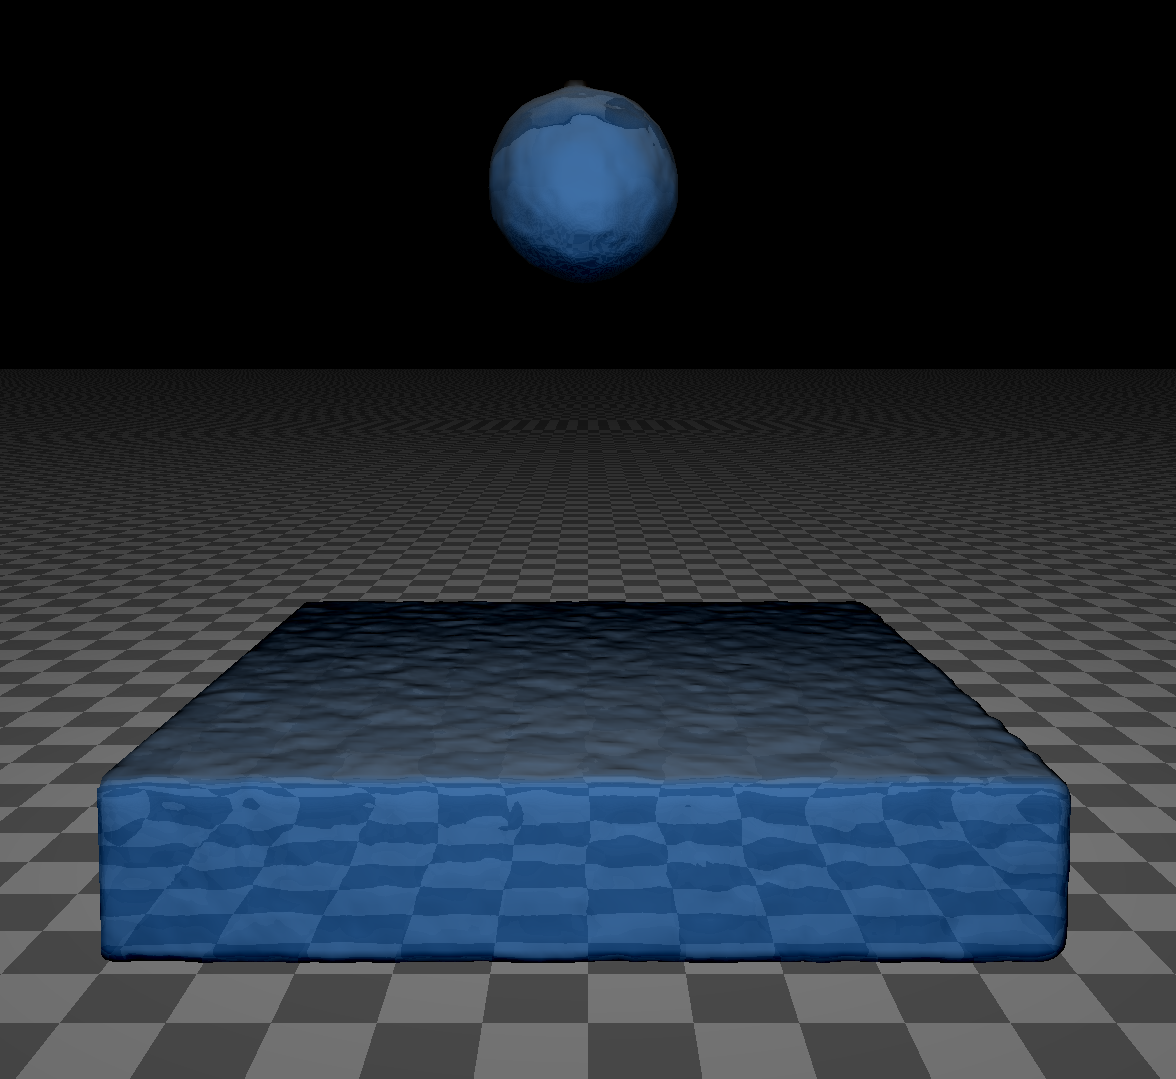
\includegraphics[width=6cm]{balldrop_cropped2/pbf0.png}
    \end{minipage}
    \begin{minipage}[t]{.42\linewidth}
        \centering
        \vspace{0pt}
        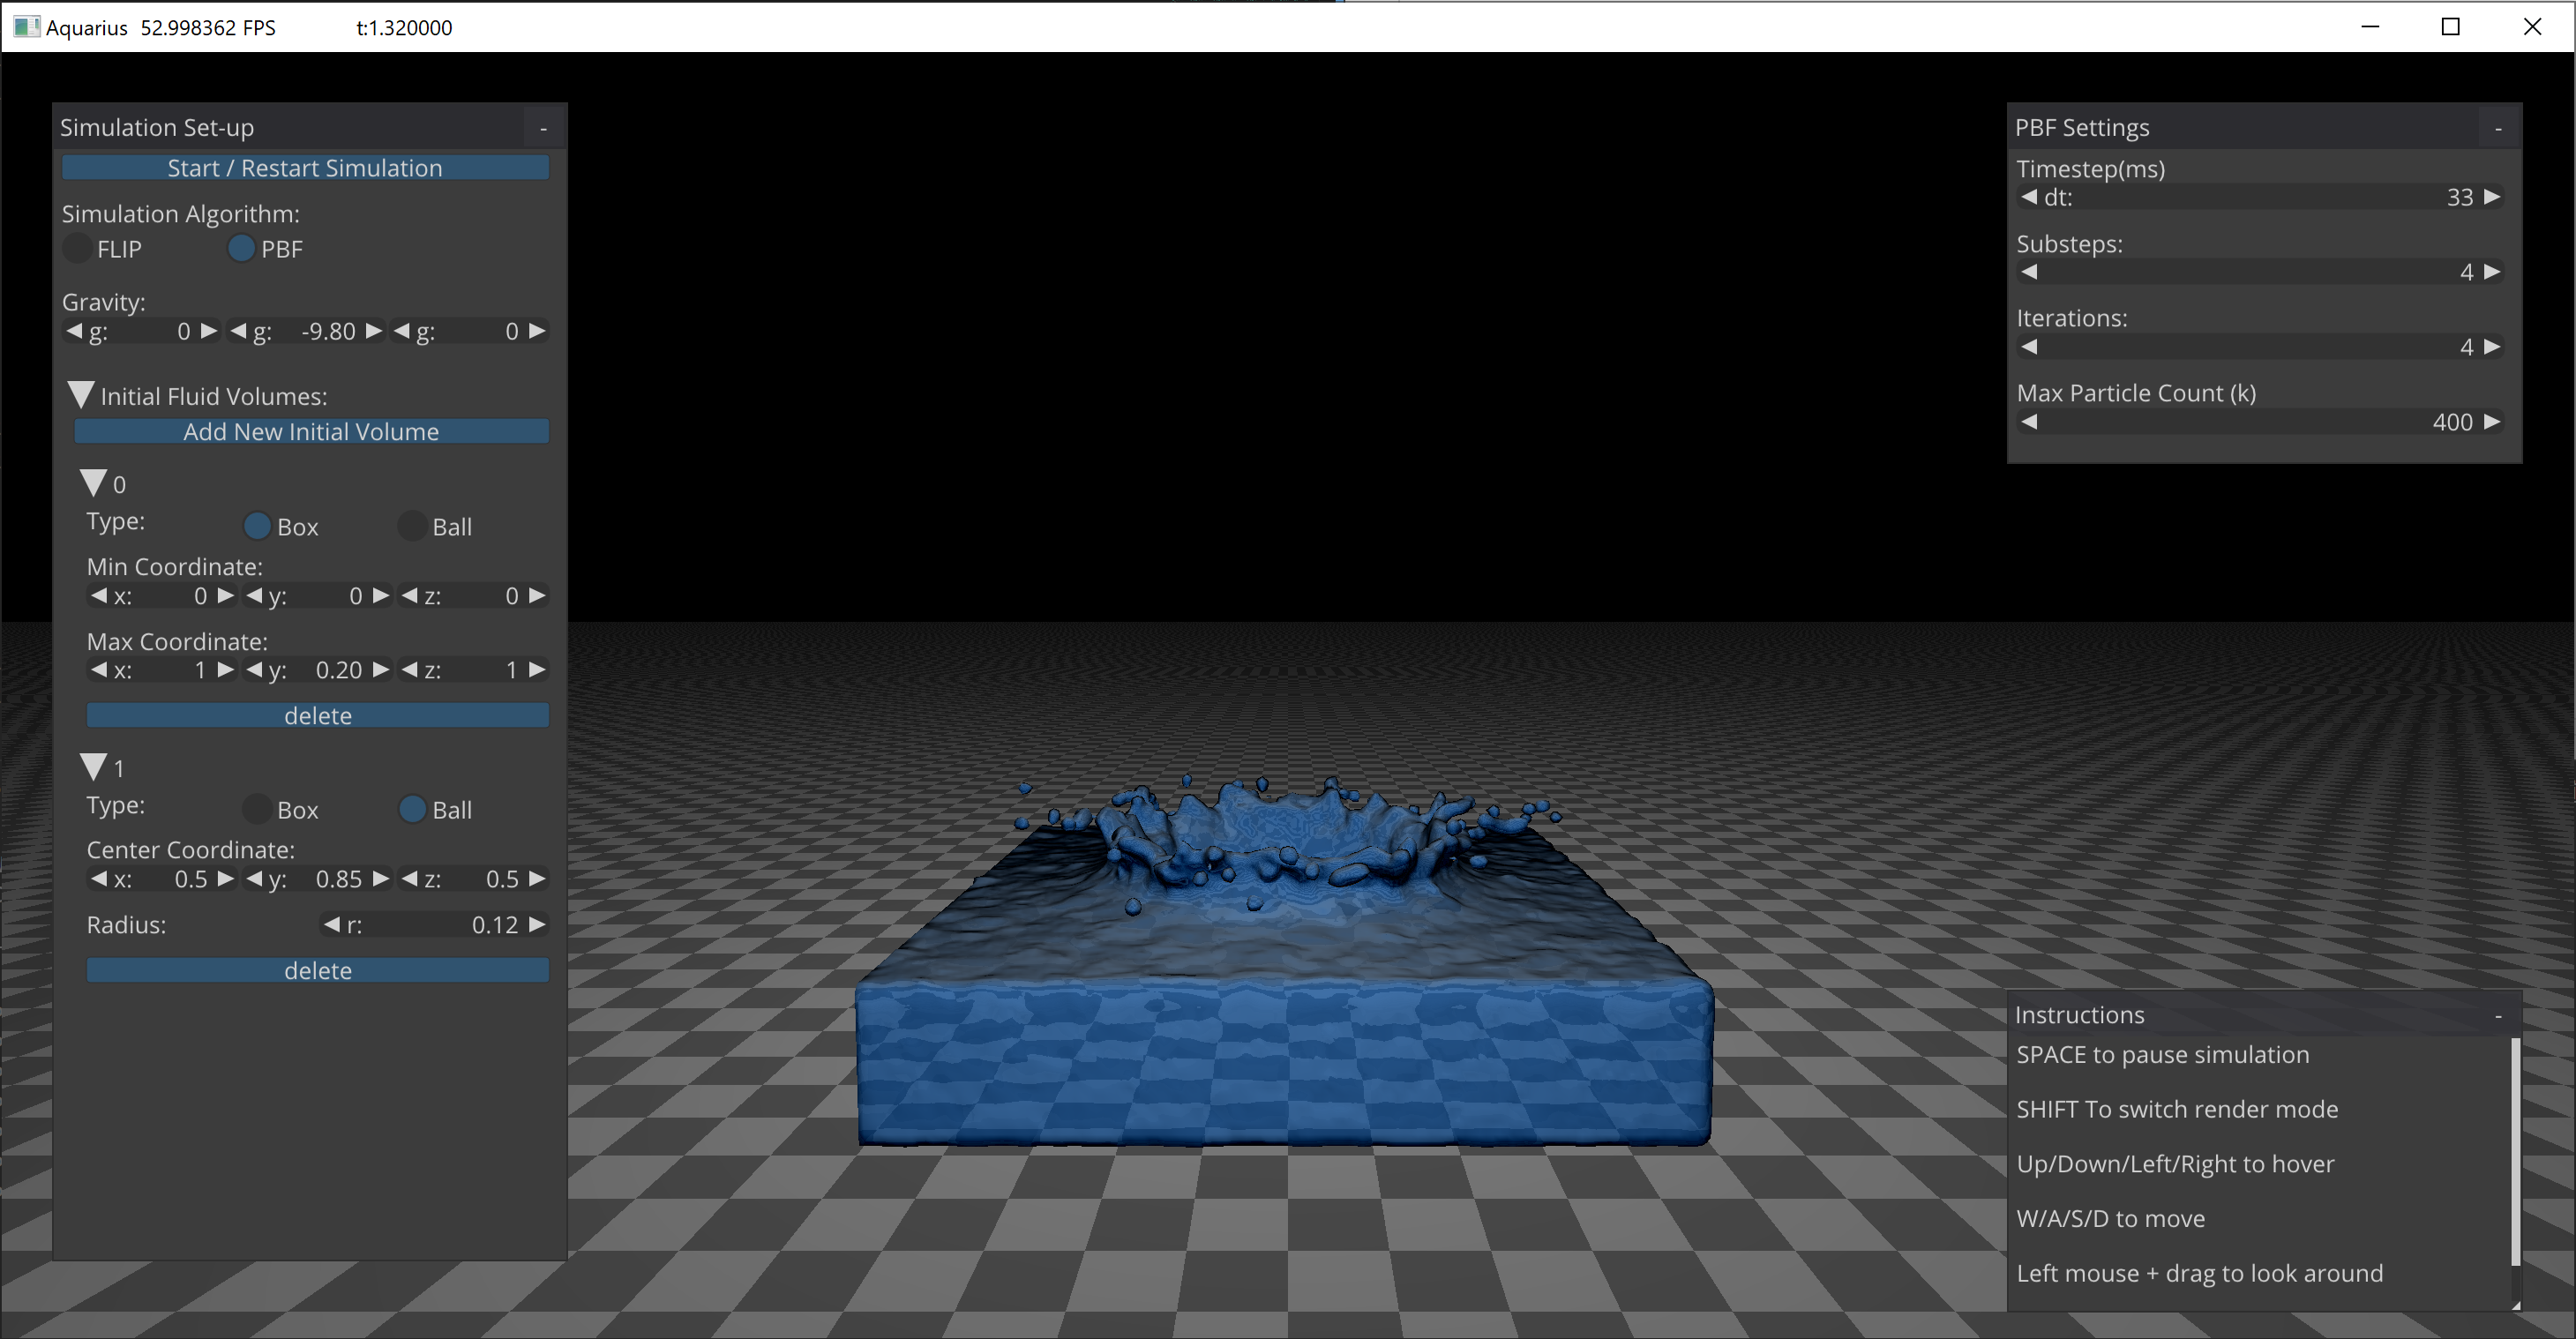
\includegraphics[width=6cm]{balldrop_cropped2/pbf1.png}
    \end{minipage}

    \vspace{0.5cm}

    \begin{minipage}[t]{.42\linewidth}
        \centering
        \vspace{0pt}
        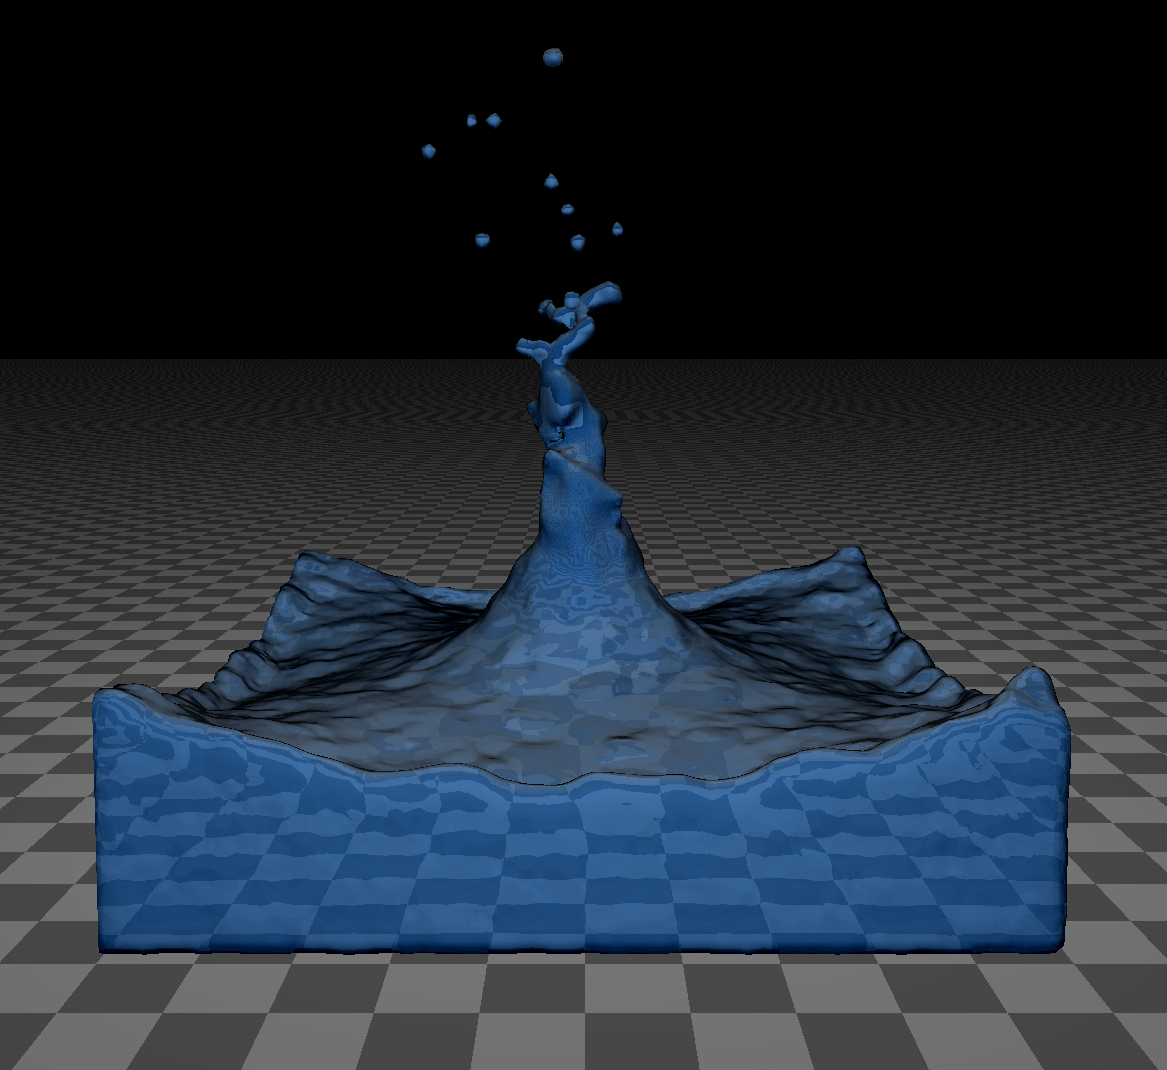
\includegraphics[width=6cm]{balldrop_cropped2/pbf2.png}
    \end{minipage}
    \begin{minipage}[t]{.42\linewidth}
        \centering
        \vspace{0pt}
        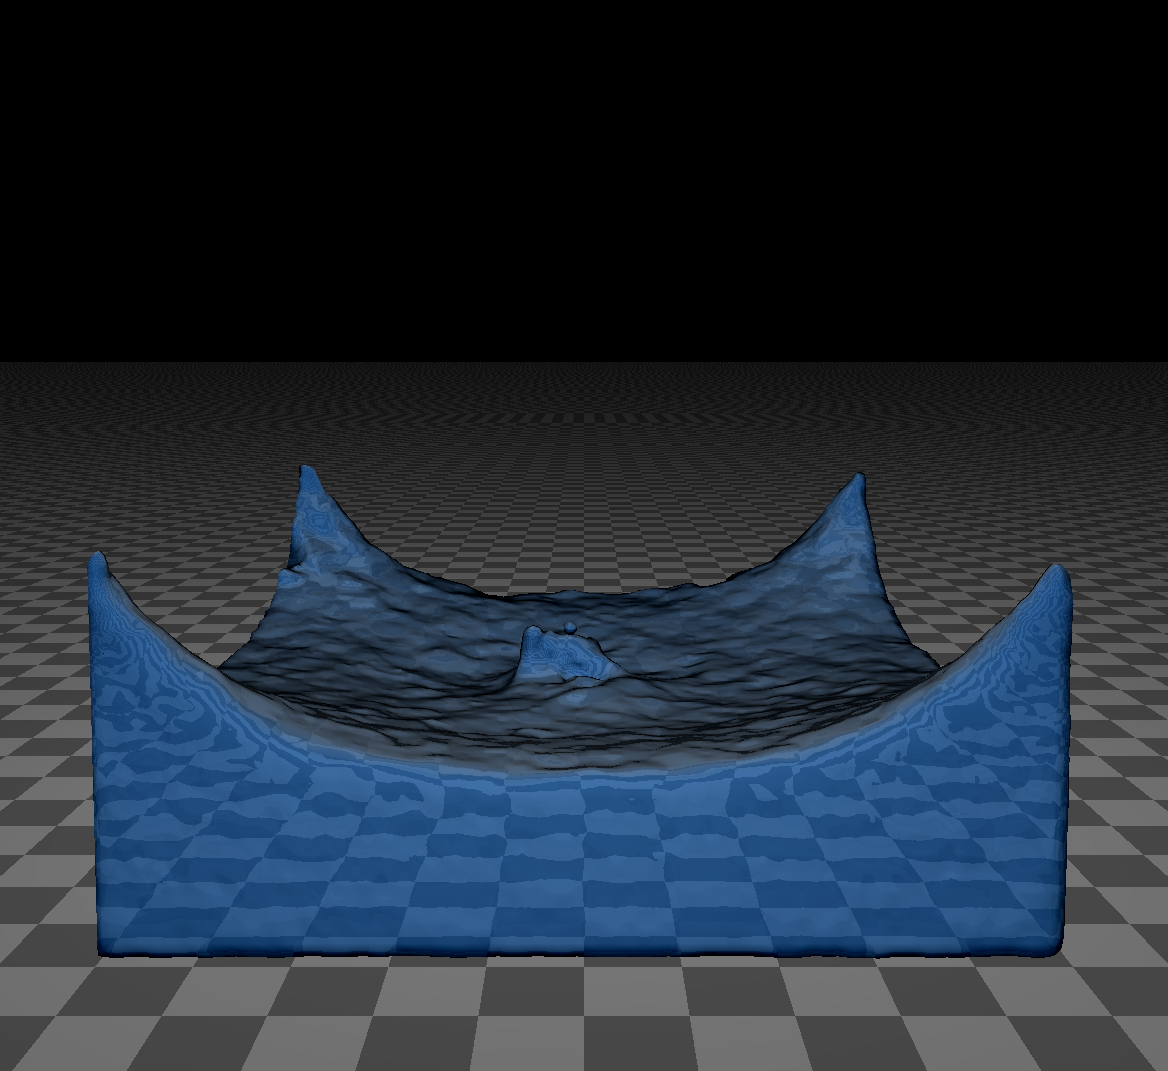
\includegraphics[width=6cm]{balldrop_cropped2/pbf3.png}
    \end{minipage}

    \caption{Same simulation as figure \ref{figure ball drop single}, except in PBF}
    \label{figure ball drop pbf}
\end{figure}
